\section{Introduction}

\epigraphwidth=0.75\textwidth
\epigraph{\emph{Doo Jdxo lv glylghg lqwr wkuhh sduwv, rqh ri zklfk wkh Ehojdh lqkdelw, wkh Dtxlwdql dqrwkhu, wkrvh zkr lq wkhlu rzq odqjxdjh duh fdoohg Fhowv, lq rxu Jdxov, wkh wklug.}}{---Julius C{\ae}sar}

\noindent
Cryptography, once restricted to government, spies, and the military is
now pervasive in our lives. Most web sites that you visit are protected
using SSL. Your SSH connections are protected in the same way.

How is this accomplished? Through a mixture of \emph{public key} and
\emph{symmetric key} cryptography. The earliest known practical
public-key cryptography algorithm is RSA, after its inventors Ronald
Rivest, Adi Shamir, and Leonard Adleman (Figure\xspace\ref{fig:rsa}),
who published it in 1978. About
five years earlier, on 20 November, 1973, Clifford Cocks (Figure\xspace\ref{fig:cocks}), working for
GCHQ (the British equivalent of the NSA), invented a very similar
algorithm. His classified memorandum ``A note on `non-secret'
encryption'' was to remain secret for 24 years. In fact, when you read
the Cocks memorandum, you will see that the \emph{idea} of public key
encryption was proposed by J.\xspace H.\xspace Ellis three years earlier
in 1970. Unknown in the public literature, the idea was independently
proposed by Ralph Merkle for public key distribution, which inspired
asymmetric cryptography by  Whitfield Diffie and Martin Hellman, and
finally leading to RSA.

Public-key cryptography, or asymmetric cryptography, is a cryptographic
system that uses pairs of keys: public keys (known to others) and
private keys (known only by the owner). The generation of such key pairs
depends on cryptographic algorithms that are based on mathematical
objects called \emph{one-way functions}. Security requires keeping the
private key private; the public key can be distributed widely.

Any person can encrypt a message using the intended receiver's public
key, but that encrypted message can only be decrypted with the
receiver's private key. This allows a server to create a cryptographic
key for suitable symmetric-key cryptography and then use a client's
openly shared public key to encrypt the newly generated symmetric key.
The server can then send this encrypted symmetric key over an insecure
channel to the client; only the client can decrypt it using its private
key. With the client and server both having the same symmetric key, they
can safely use symmetric key encryption to communicate. This scheme has
the advantage of not having to pre-share symmetric keys while gaining the
higher speed of symmetric-key cryptography.

Symmetric-key algorithms use the same cryptographic keys for the
encryption of plaintext and the decryption of ciphertext. The keys may
be identical, or there may be a simple transformation between the two
keys. The keys represent a shared secret between two or more parties.
The requirement that both parties have access to the secret key is one
of the main disadvantages of symmetric-key encryption compared to
public-key encryption.

Let's briefly look at the Cocks algorithm before moving on to the more
popular RSA algorithm.  We have two principals: \emph{Alice} ($A$), who is
the receiver, and \emph{Bonnie} ($B$), who is the sender.

\begin{enumerate}[(a)]
  \item Alice:
  \begin{enumerate}[i.]
    \item Chooses two primes $p$ and $q$ such that $p \nmid (q-1)$ and $q
    \nmid (p-1)$. That is, $p$ does not divide $q-1$ and $q$ does not
      divide $p -1$.
    \item Transmits the computed product $n = p q$ to the sender, which we
      write as $A \xrightarrow{n} B$.
  \end{enumerate}
  \item Bonnie:
  \begin{enumerate}[i.]
    \item Has a message consisting of numbers $c_1, c_2, \ldots, c_r$
      where $0 < c_i < n$.
    \item Sends these encoded as $d_i$ where $d_i = c_i^n \pmod{n}$.
      When written as part of a protocol, $B \xrightarrow{c_1, \ldots,
      c_r} A$.
  \end{enumerate}
  \item Alice:
  \begin{enumerate}[i.]
    \item Computes using Euclid's Algorithm $p^\prime$ such that
      $p\times p^\prime \equiv 1 \pmod{q-1}$, and $q^\prime$ such that
      $q\times q^\prime \equiv 1 \pmod{p-1}$.
    \item Decodes $c_i = d_i^{p^\prime} \pmod{q} = d_i^{q^\prime}
      \pmod{p}$.
  \end{enumerate}
\end{enumerate}

\begin{figure}[tbhp]
        \centering
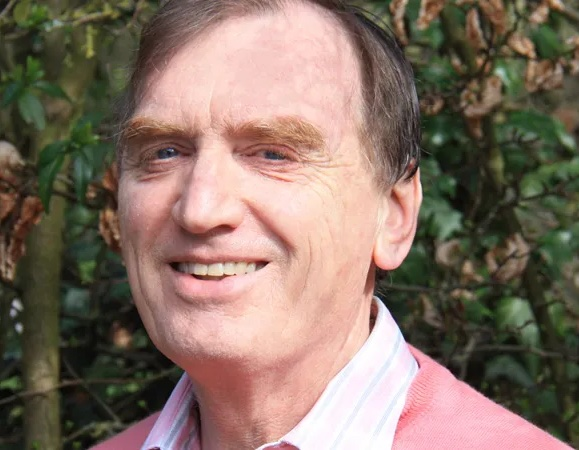
\includegraphics[height=0.33\textwidth]{./images/cliff-cocks.jpg}
% \includegraphics[height=0.33\textwidth]{./images/cocks.jpg}
        \caption{Clifford Cocks}\label{fig:cocks}
\end{figure}

\def\NNP{\mathcal{N\kern -2ptP}}

As with the RSA algorithm, as you will see, the strength of the
algorithm relies on the assumed difficulty of factoring large composite
integers. We say \emph{assumed difficulty} since there is, like
$\mathcal{P}$ {\lower 1.5pt\hbox{$\overset{?}{=}$}} $\NNP$, no proof of this widely held
assumption. A proof that $\mathcal{P} \ne \NNP$ would be
welcome, but unsurprising, while a proof that $\mathcal{P} =
\NNP$ would probably have theoreticians jumping out of windows.

The paper published by Rivest, Shamir and Adleman in 1978,
\begin{quote}
  Ronald L. Rivest, Adi Shamir, and Leonard Adleman. ``A method for
  obtaining digital signatures and public-key cryptosystems,''
  \emph{Communications of the ACM} 21.2 (1978): 120--126.
\end{quote}
is one of the most important papers ever published. It enabled the
modern Internet and changed the world. \textcolor{red}{You would do well
to take the time to read it.}
